\documentclass[12pt]{beamer}

\usepackage{amsmath}
\usepackage{amssymb}
\usepackage{graphics, subfigure}
%\pagestyle{empty}
\usepackage{slashbox}
\usepackage{colortbl}
\usepackage{color}
\usepackage{tabu}

\newcommand{\hilight}[1]{\colorbox{yellow}{#1}}
%\usepackage{soul}

\usepackage{graphicx}
\usetheme[secheader]{Madrid}
\usefonttheme[stillsansserifsmall]{serif}
\usefonttheme[onlylarge]{structurebold}
\usecolortheme[RGB={10,120,100}]{structure}
\setbeamertemplate{navigation symbols}{}

%\input{defs}

\newtheorem*{remark}{Remark}
\author[]{%
  Thibaut Astic
  }
\title[]{Application of compressive sensing ideas to Static Electromagnetic Geophysics}
\date[]{EOSC 513 2017: Project \\ https://github.com/thast/EOSC513}

% \titlegraphic{\includegraphics[width=22mm]{figures/Kinv}}

% \begin{figure}[h!]
%     % \begin{center}
%     \centering
%     \includegraphics[width=80mm]{figures/Eigen}
%     % \end{center}
%     \caption{Real part of eigenvalues of preconditioned matrix $\re{\mathcal{P}_{\rm schurMH}^{-1} \mathcal{K}_{\rm MH}}$ (imaginary parts small)}
% \end{figure}

% \institute[]{University of British Columbia}

\definecolor{darkgreen}{rgb}{0,0.5,0}
\definecolor{darkyellow}{rgb}{.8,.6,.04}
\newcommand{\gr}[1]{\textcolor{darkgreen} {#1}}
\newcommand{\wh}[1]{\textcolor{white}     {#1}}
\newcommand{\dy}[1]{\textcolor{darkyellow}{#1}}
\newcommand{\yb}[1]{\colorbox {yellow}    {#1}}
\newcommand{\re}[1]{{\textcolor{red}       {#1}}}
\newcommand{\bl}[1]{{\textcolor{blue}{#1}}}
\newcommand{\w}[1]{{\textcolor{white}{#1}}}

\newcommand{\RE}[1]{{\bf\textcolor{red}       {#1}}}
\newcommand{\GR}[1]{{\bf\textcolor{darkgreen} {#1}}}
\newcommand{\DY}[1]{{\bf\textcolor{darkyellow}{#1}}}
\newcommand{\BL}[1]{{\bf\textcolor{blue}{#1}}}
\newcommand{\ssec}[1]{{\bf #1}}
\newcommand{\rsec}[1]{{\bf\color{red}       #1}}
\newcommand{\bsec}[1]{{\bf\color{blue}      #1}}
\newcommand{\gsec}[1]{{\bf\color{darkgreen} #1}}
\newcommand{\dom}{\mbox{\sf dom}}

\newcommand{\curl}{\ensuremath{\nabla\times\,}}
\renewcommand{\div}{\nabla\cdot\,}
\newcommand{\grad}{\ensuremath{\nabla}}

\usepackage[utf8]{inputenc}
\usepackage{array}
\usepackage[export]{adjustbox}
\usepackage{wrapfig}



\newcommand{\R}{\mathbb{R}}
\newcommand{\minim}{\mathop{\mathrm{minimize}}}
\newcommand{\minimize}[1]{\displaystyle\minim_{#1}}
\newcommand{\maxim}{\mathop{\mathrm{maximize}}}
\newcommand{\maximize}[1]{\displaystyle\maxim_{#1}}
\newcommand{\st}{\mathop{\mathrm{subject\ to}}}
\newcommand{\Null}{\mathop{\mathrm{Null}}}
\newcommand{\A}{\mathcal{A}}
\newcommand{\I}{\mathcal{I}}
\newcommand{\kns}{\mathcal{K}_{\rm NS}}
\newcommand{\km}{\mathcal{K}_{\rm M}}
\newcommand{\kc}{\mathcal{K}_{\rm C}}

\newcommand{\aheader}[2]{\action{#2}}
% first argument: slide number to appear from, second argument: content of header
\newcommand{\hiddencell}[2]{\action<#1->{#2}}
% first argument: slide number to appear from, second argument: content of cell


\begin{document}

\begin{frame}
  \titlepage
\end{frame}



\title{Sparse GN update}
  \begin{frame}<beamer>
    \frametitle{Outline}
    \tableofcontents
  \end{frame}

\AtBeginSection[]
{
  \begin{frame}<beamer>
    \frametitle{Outline}
    \tableofcontents[currentsection]
  \end{frame}
}


\section{Motivation}
\begin{frame}{DC Resistivity Survey}

\begin{columns}
\begin{column}{0.5\textwidth}

\begin{figure}[t!]
    % \begin{center}
    %\centering
    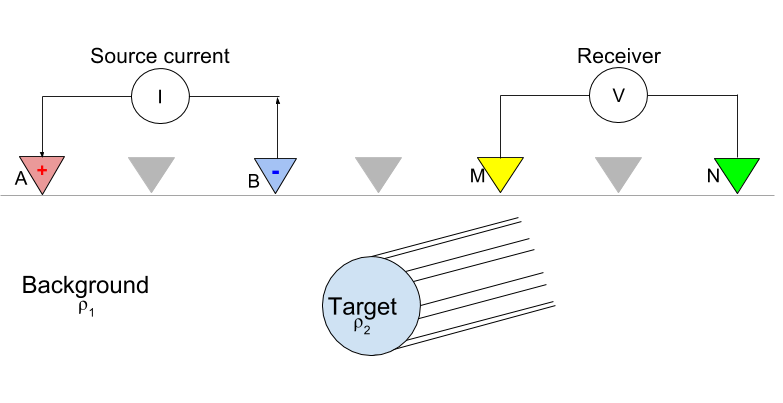
\includegraphics[width=60mm, left]{figures/DCR_Setup_Cylinder.png}
    % \end{center}
\end{figure}

Currents are injected to the earth. Theirs flow will be distorted depending upon the conductivity contrast in the earth
These changes can be measurable on the surface electrodes. 
\href{https://notebooks.azure.com/library/em_apps}{\color{blue} Interactive notebooks}

\end{column}
\begin{column}{0.5\textwidth}
\begin{figure}[t!]
    % \begin{center}
    %\centering
    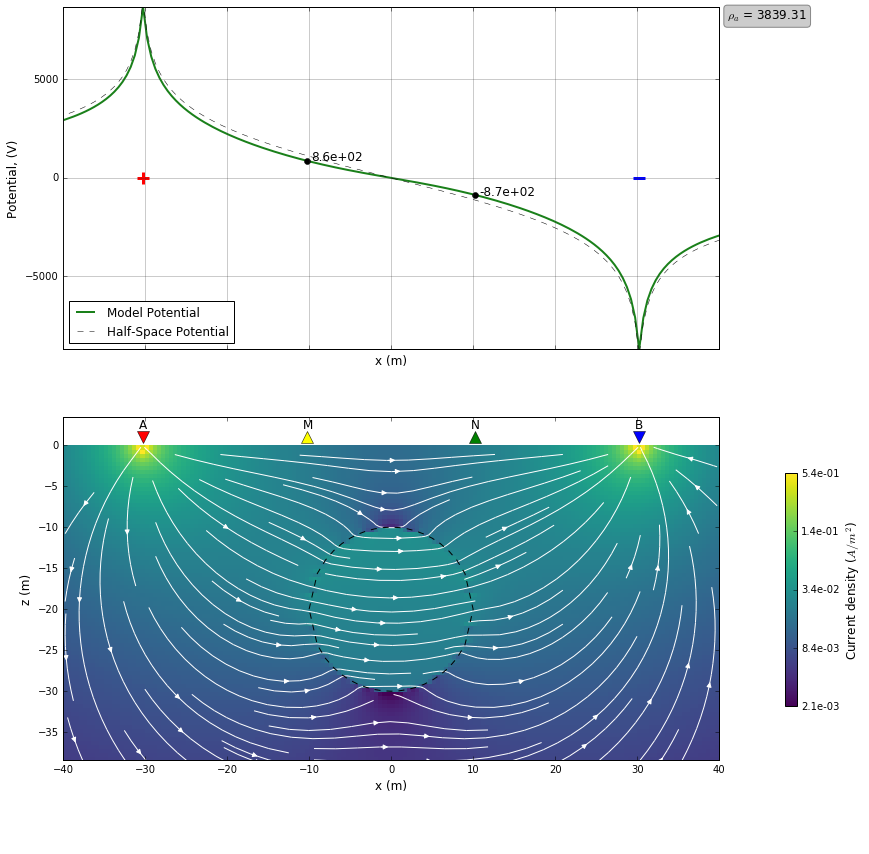
\includegraphics[width=60mm, left]{figures/DC_survey.png}
    % \end{center}
\end{figure}
\end{column}

\end{columns}

\end{frame}

\begin{frame}{DCR Physics: Maxwell's equations}

\begin{figure}[t!]
    % \begin{center}
    %\centering
    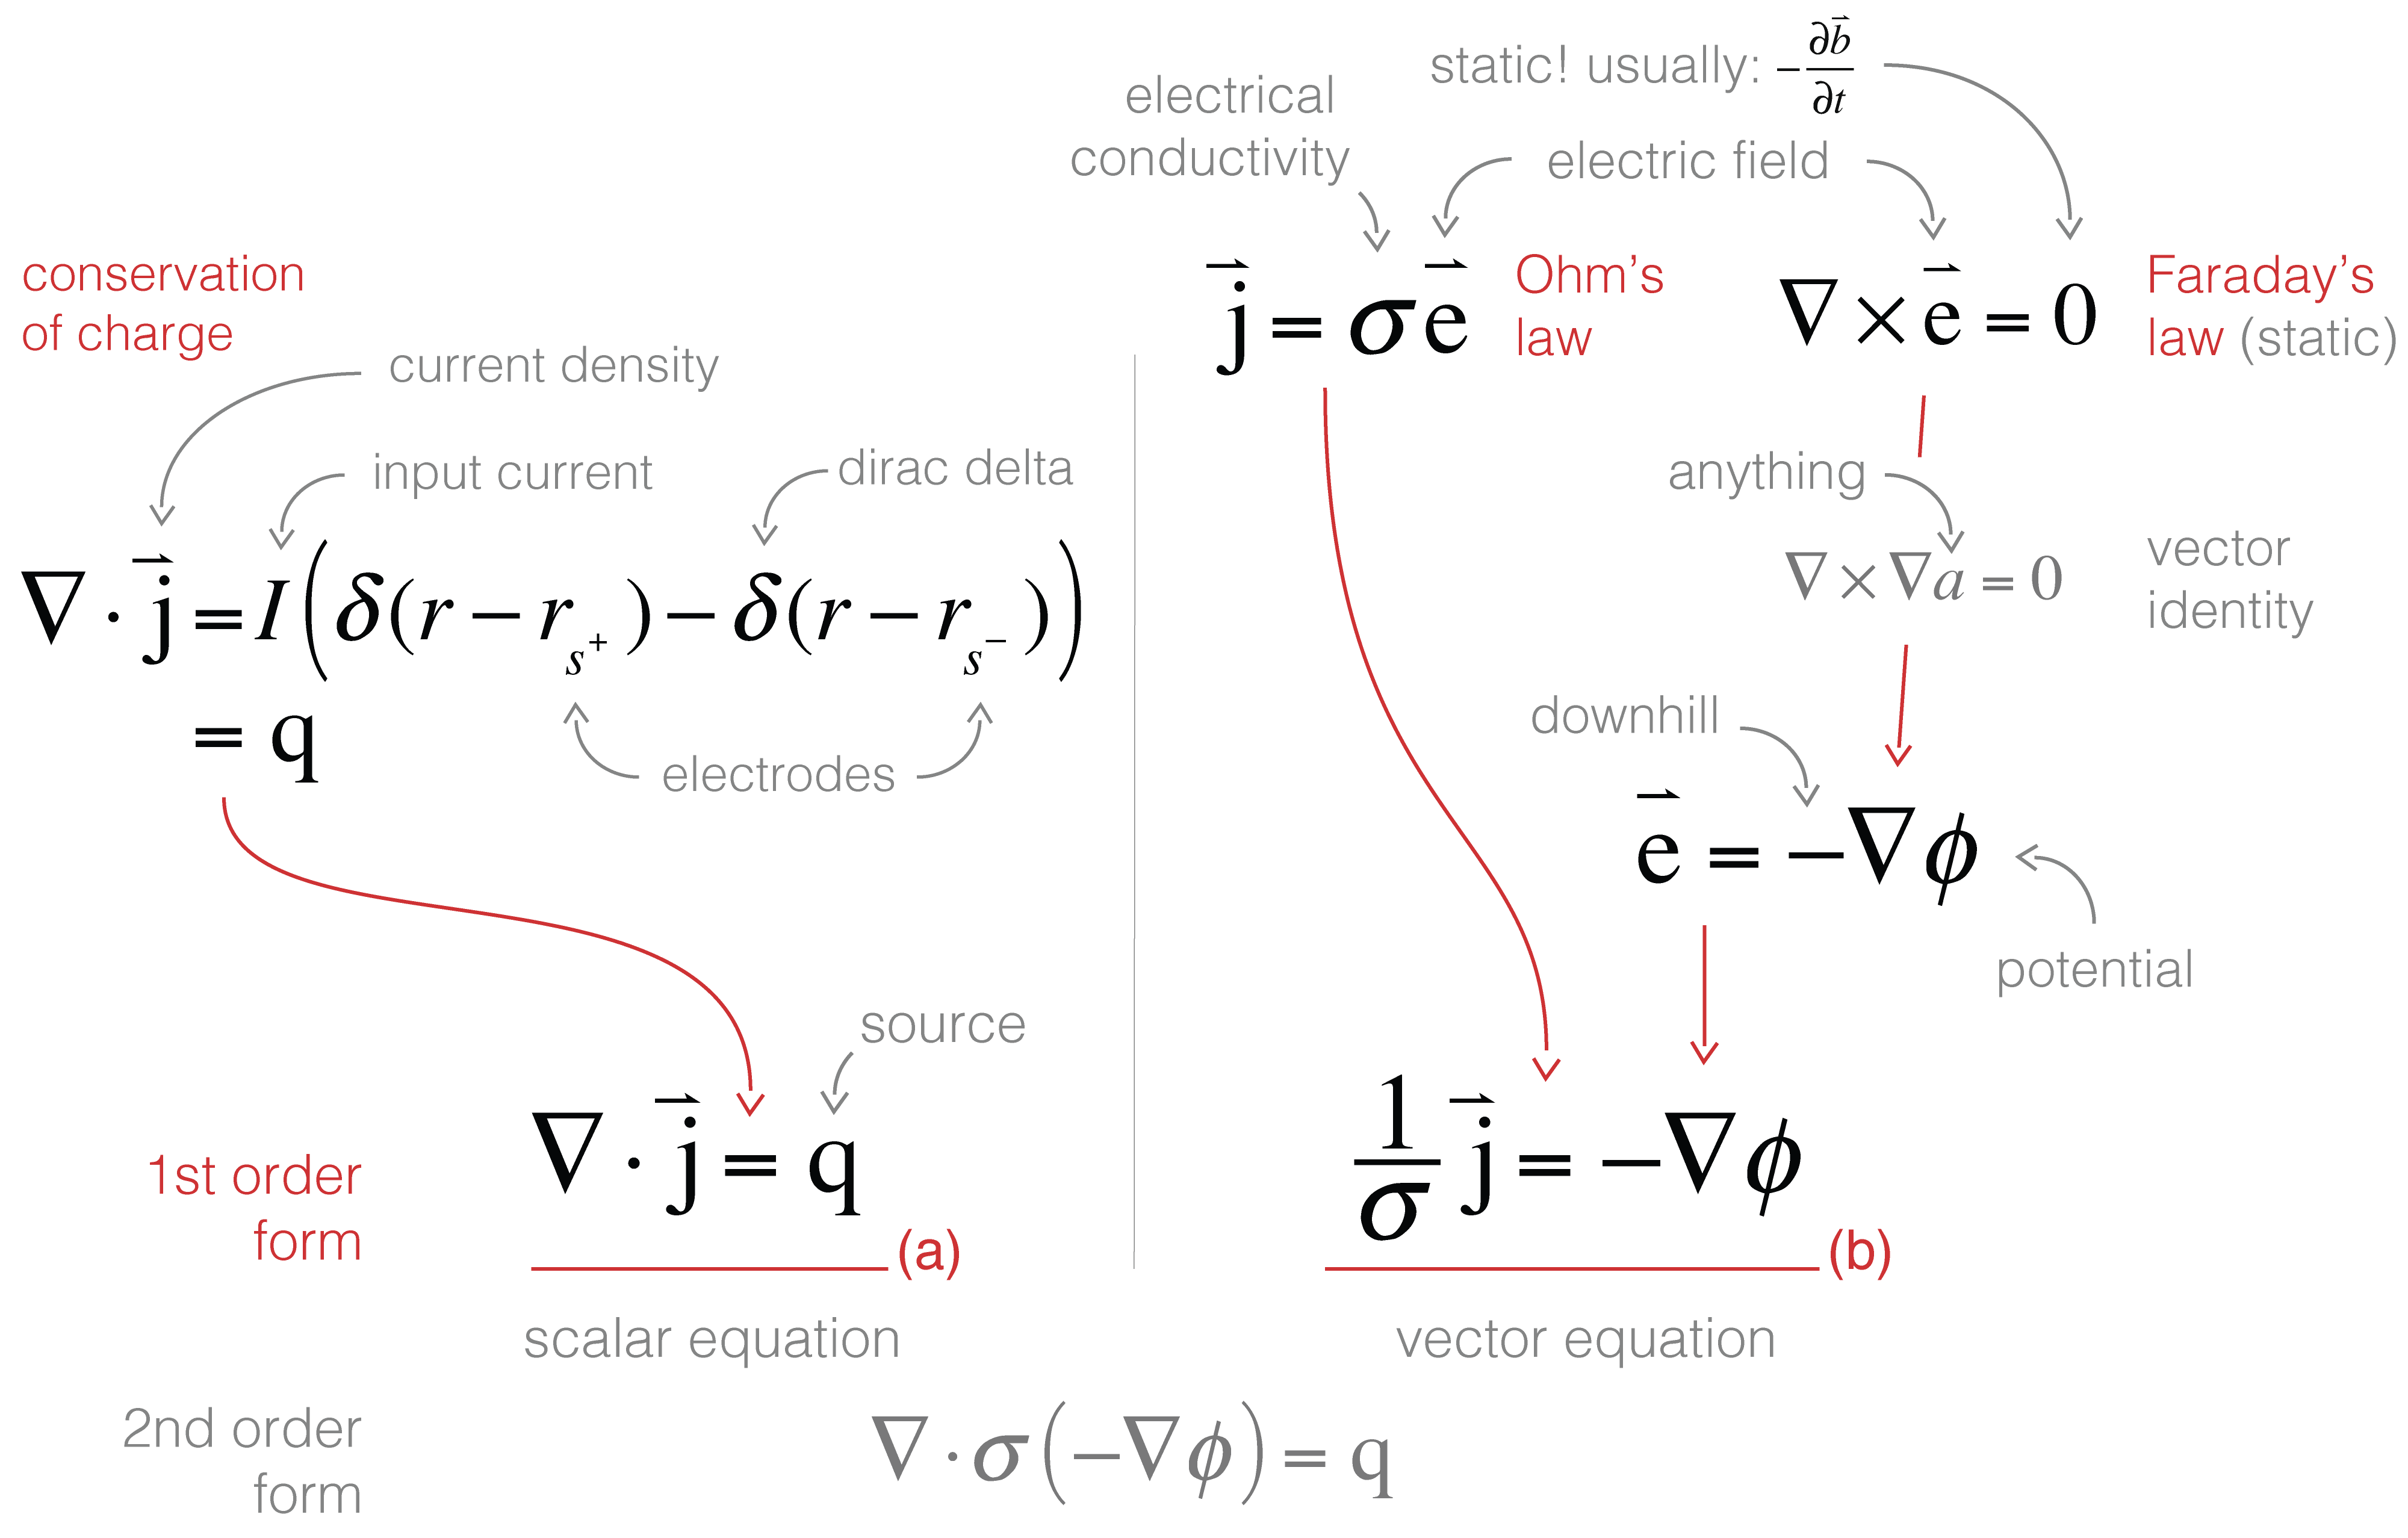
\includegraphics[width=80mm]{figures/DCEquations.png}
    % \end{center}
\end{figure}

\href{http://tutorials.simpeg.xyz/content/pixelsandtheirneighbors.html}{\color{gray} Rowan Cockett, Lindsey J. Heagy, and Douglas W. Oldenburg (2016). ”Pixels and their neighbors: Finite volume.” The Leading Edge, 35(8), 703–706. doi: 10.1190/tle35080703.1}

\end{frame}

\begin{frame}{DCR: inverse Problems}

\begin{itemize}
  \item SimPEG: open-source python package for EM Geophysics
  \item discretize using a Finite Volume Formulation
  \begin{align}
  \text{diag}(\mathbf{v})
  \mathbf{D}
  \mathbf{M}_f(\sigma^{-1})^{-1}
  \mathbf{D}^\top
  \text{diag}(\mathbf{v})
  \boldsymbol{\phi} =
  \mathbf{q}.
  \end{align}
  \item Solve for $m = \ln(\sigma)$ to ensure positivity of conductivity
  \item Use a beta-cooling strategy for the regularizer's weight
\end{itemize}

\begin{align}
f(m) &= \frac{1}{2} \sum_{i=1}^{N_s} ||P_iA(m)^{-1}q_i-d_i||_2^2 + \beta R(m) \\
f(m) & = \frac{1}{2} ||PA(m)^{-1}Q-D||_F^2  +\beta R(m)
\end{align}
Usually:
\begin{align}
R(m) = \frac{1}{2} ||W(m-m_{ref})||_2^2
\end{align}

\end{frame}

\begin{frame}{DCR: Solving the inverse problem}

\begin{itemize}
  \item solve a linearized problem
  \item Inexact Gauss-Newton steps
\end{itemize}

\begin{align}
f(m) &= \frac{1}{2} ||r(m)||_2^2 + \beta ||W(m-m_{ref})||_2^2 \\
f(m+\delta m) &= \frac{1}{2} ||r(m)+J(m)\delta m||_2^2 + \beta ||W(m+\delta m-m_{ref})||_2^2
\end{align}

%Solve:

\begin{align}
(J^TJ+\beta W^TW)\delta m = -J^Tr(m) - \beta W^TW(m-m_{ref})
\end{align}

Update m: $m_{k+1} = m_k+\alpha \delta m$ s.t $f(m_{k+1}) < \gamma f(m_{k})$

\end{frame}

\begin{frame}{DCR: inverse Problems Results}


\begin{figure}[t!]
    % \begin{center}
    %\centering
    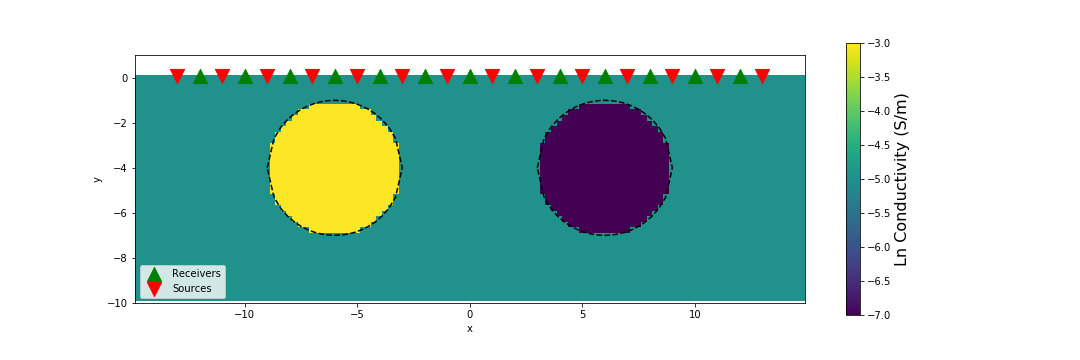
\includegraphics[width=70mm]{figures/initialmodel.png}
    \caption{Initial model and survey}
    % \end{center}
\end{figure}

  
\begin{figure}[t!]
    % \begin{center}
    %\centering
    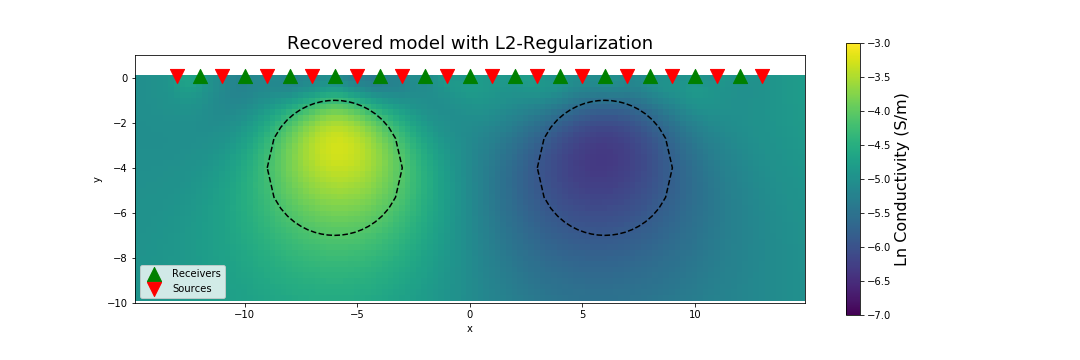
\includegraphics[width=70mm]{figures/recoveredModel.png}
    \caption{Recovered model with L2 Regularization}
    % \end{center}
\end{figure}

\end{frame}

\begin{frame}{Problematic}

\begin{itemize}
  \item The cost of inverting DC data is mainly driven by the number of sources:
  \begin{itemize}
    \item Can we decrease this cost? What is the price to pay?
  \end{itemize}
\vspace{20pt}
  \item The diffusive nature of the physics behind DCR and the L2-Regularization are promoting smooth update
  \begin{itemize}
    \item Can we, in some space, promote sparsity for such a problem?
  \end{itemize}
\end{itemize}

\end{frame}

\section{Source Encoding}

\begin{frame}{Reducing the number of Sources}

We start to try one of the basic idea of Compressive Sensing by using simultaneous sources.

\begin{align}
f(m) & = \frac{1}{2} ||PA(m)^{-1}QW-DW||_F^2  +\beta R(m)
\end{align}

W a random gaussian matrix of size $N_s \times N_{ss}$ with $N_{ss}<<N_s$ \\
The Gauss-Newton step subproblem's size is then reduced by a factor $\frac{N_{s}}{N_{ss}}$

We have then experiment several strategies for updating W.

\end{frame}


\begin{frame}{Updating W}

\begin{figure}

  \subfigure{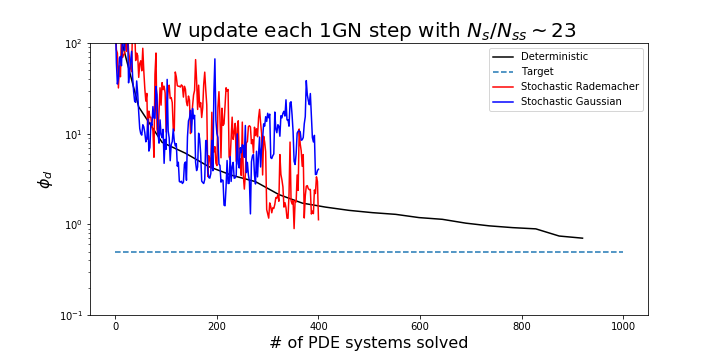
\includegraphics[width=50mm]{figures/W_update_each_1GN_steps_with_1_sources.png}}
  \subfigure{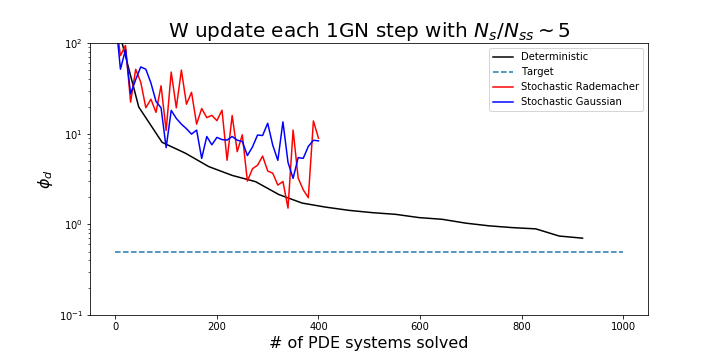
\includegraphics[width=50mm]{figures/W_update_each_1GN_step_with_5_sources.png}}
  \subfigure{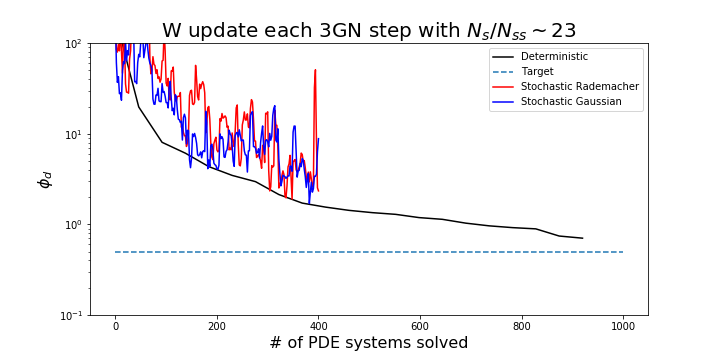
\includegraphics[width=50mm]{figures/W_update_each_3GN_step_with_1_source.png}}
  \subfigure{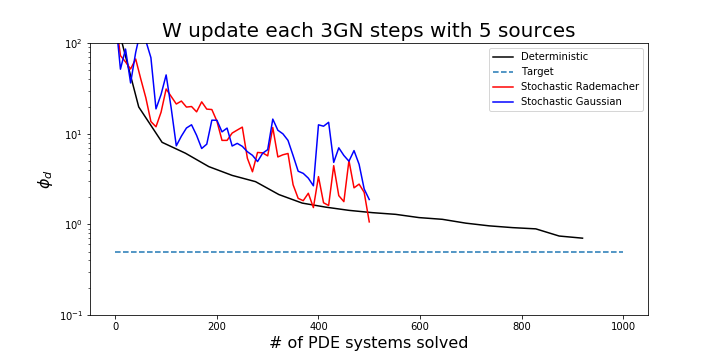
\includegraphics[width=50mm]{figures/W_update_each_3GN_steps_with_5_sources.png}}


\end{figure}

\end{frame}

\section{Sparse Gauss Newton Update}

\begin{frame}{Formulating the GN subproblem}

Original Data fitting subproblem:
\begin{align}
\text{min}_{\delta m} \frac{1}{2} ||J(m)\delta m + r(m)||_2^2 + \beta ||W(m+\delta m-m_{ref})||_2^2
\end{align}

%\begin{align}
%(J^TJ+\beta W^TW)\delta m = -J^Tr(m) - \beta W^TW(m-m_{ref})
%\end{align}

%\begin{align}
%(J^TJ+\beta W^TW)\delta m = -J^Tr(m) - \beta W^TW(m-m_{ref})
%\end{align}

Now without the L2 penalty but a L1 constrain in some space:
\begin{align}
\text{min} ||\delta x||_1 ~\text{s.t}~ ||J(m)S^H \delta x + r(m)||^2_2 < tol
\end{align}

\begin{itemize}
\item $\delta x = S \delta m$
\item $S$ a sparsifying matrix  
\item $S^H$ the inverse transform.
\item solved using SPGL1 \\
{\color{gray} E. van den Berg and M. P. Friedlander, "Probing the Pareto frontier for basis pursuit solutions", SIAM J. on Scientific Computing, 31(2):890-912, November 2008}
%\item tolerance is chosen such that it performs at least as the L2-norm regularized problem for each GN step
\end{itemize}
\end{frame}

\begin{frame}{Choosing a sparsifying transform}
\begin{itemize}
  \item The model to recover should be sparse in some space


\begin{figure}
  \subfigure{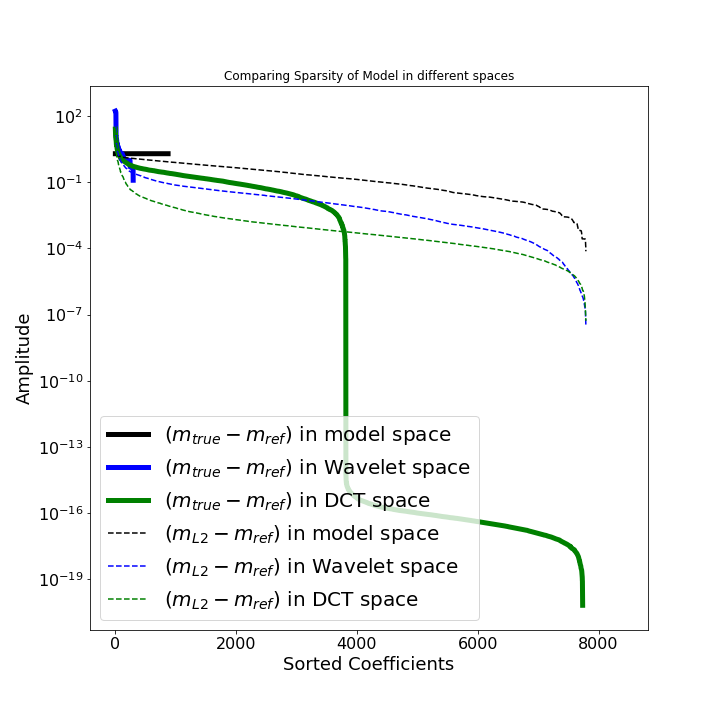
\includegraphics[width=60mm]{figures/Model_sparsity_diff_spaces.png}}
\end{figure}

\end{itemize}

\end{frame}

\begin{frame}{Choosing a sparsifying transform}
\begin{itemize}
  \item the columns of $J^T$ and $S^H$ should be incoherent
  \item The DC problem is a weighted Laplacian
  \item The eigenfunctions of the Laplacian are cosine functions


\begin{figure}
  \subfigure{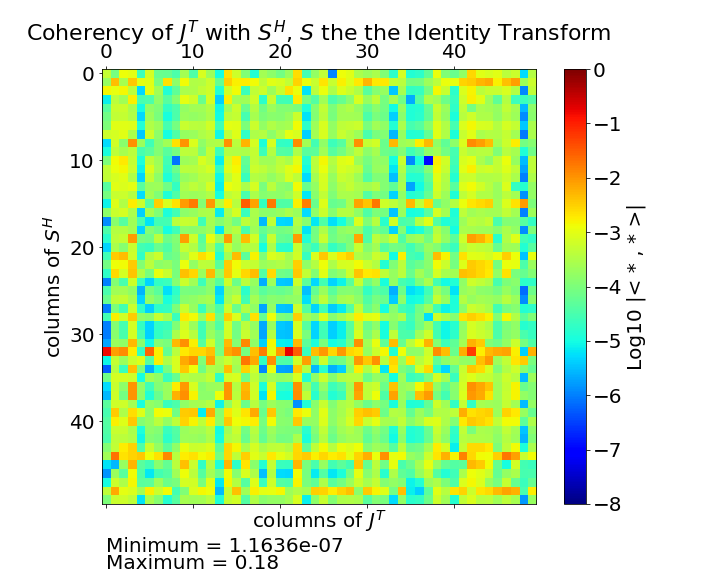
\includegraphics[width=35mm]{figures/Coherency_Identity.png}}
  \subfigure{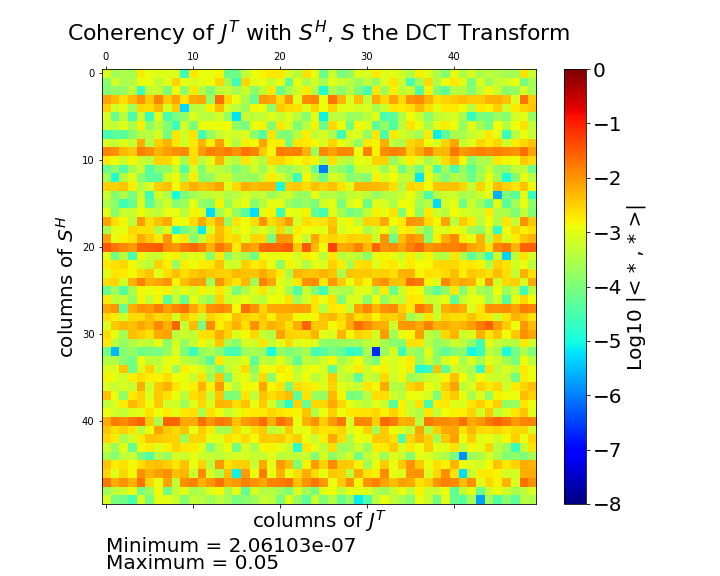
\includegraphics[width=35mm]{figures/Coherency_DCT.png}}
  \subfigure{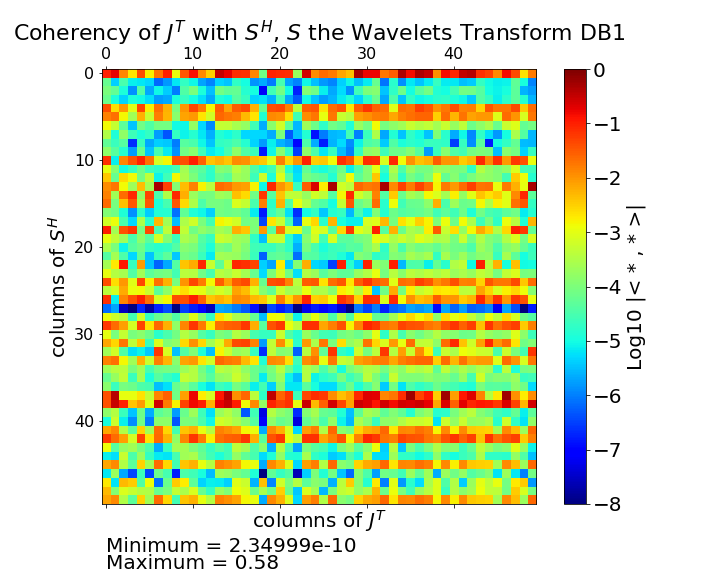
\includegraphics[width=35mm]{figures/Coherency_Wavelet.png}}
\end{figure}

\end{itemize}

\end{frame}


\begin{frame}{Recovered Models using sparse GN update: S = Identity or DCT }
\begin{itemize}
  \item Without Source Encoding
\end{itemize}
\begin{figure}
  \subfigure{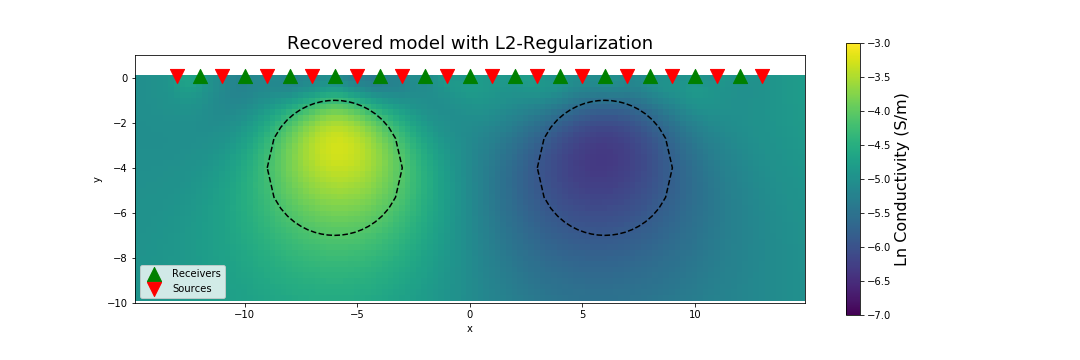
\includegraphics[width=59mm]{figures/recoveredModel.png}}
  \subfigure{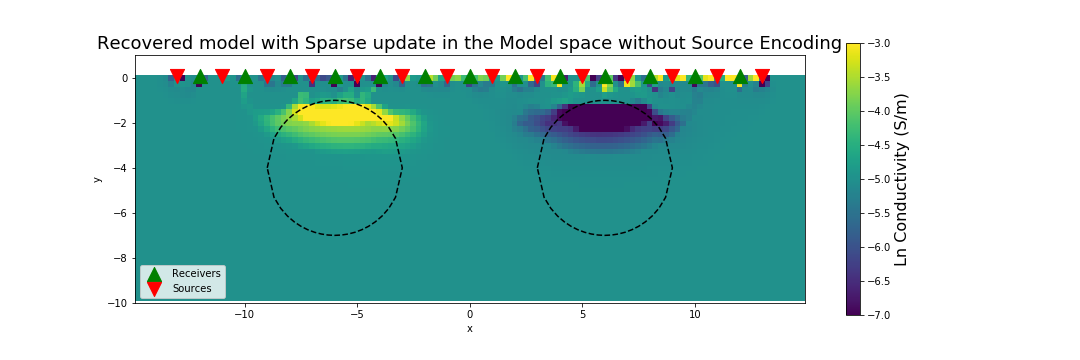
\includegraphics[width=59mm]{figures/recoveredModel_SparseId.png}}
  \subfigure{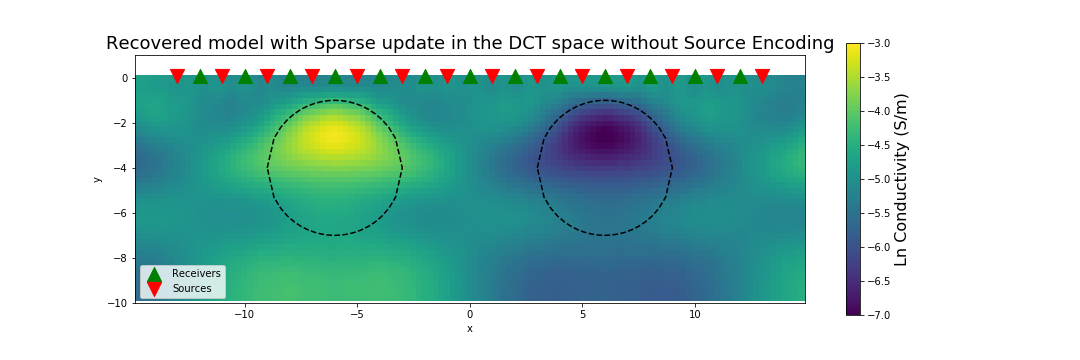
\includegraphics[width=59mm]{figures/recoveredModel_SparseDCT.png}}
  %\subfigure{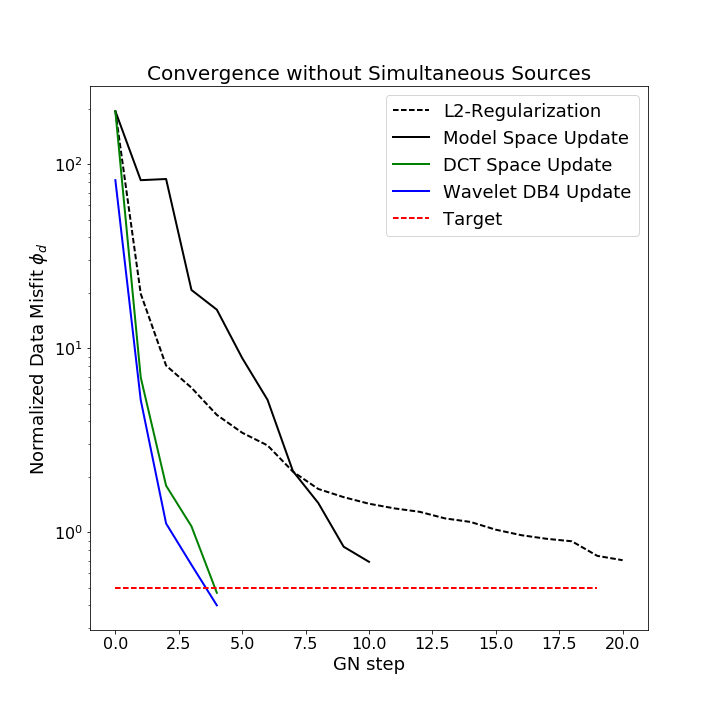
\includegraphics[width=30mm]{figures/Convergence_Sparse_withoutW.png}}

\end{figure}

\end{frame}

\begin{frame}{Recovered Models using sparse GN update in Wavelets space}
\begin{itemize}
  \item Without Source Encoding
\end{itemize}
\begin{figure}
  \subfigure{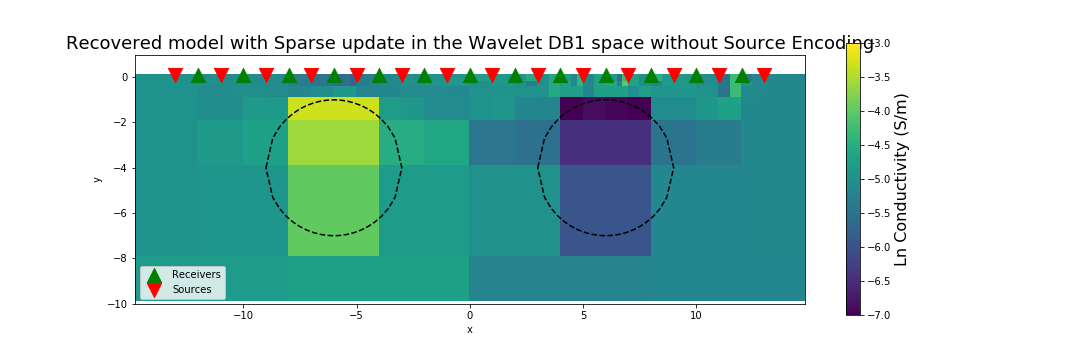
\includegraphics[width=59mm]{figures/recoveredModel_SparseWVT_DB1_withoutW.png}}
  \subfigure{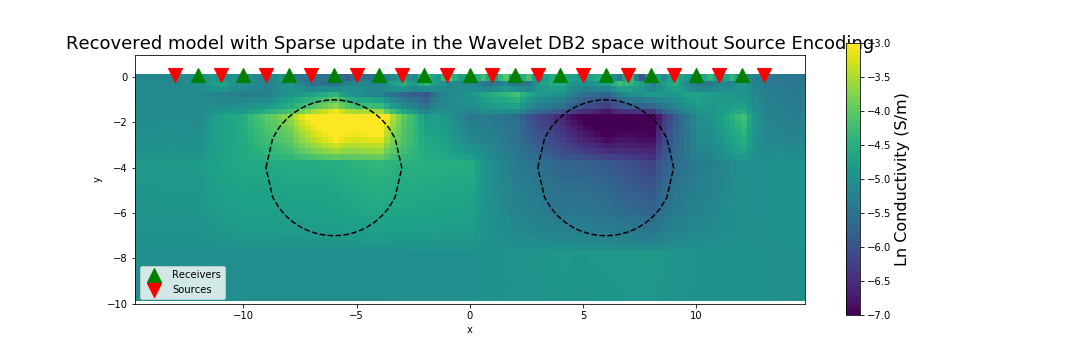
\includegraphics[width=59mm]{figures/recoveredModel_SparseWVT_DB2_withoutW.png}}
  \subfigure{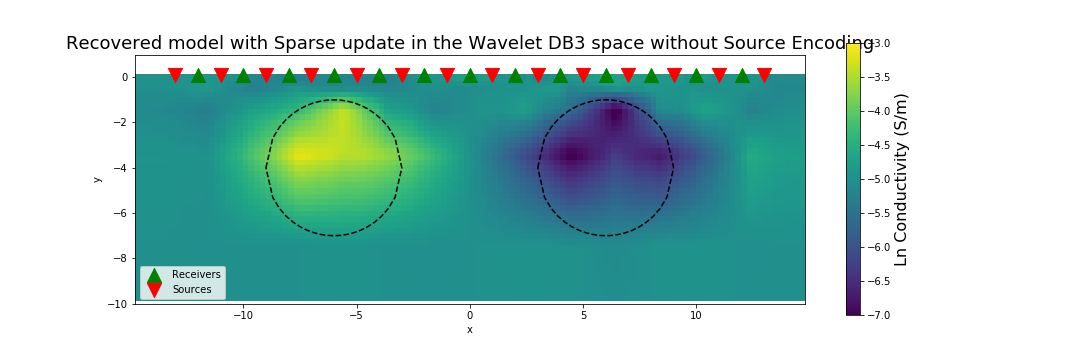
\includegraphics[width=59mm]{figures/recoveredModel_SparseWVT_DB3_withoutW.png}}
  \subfigure{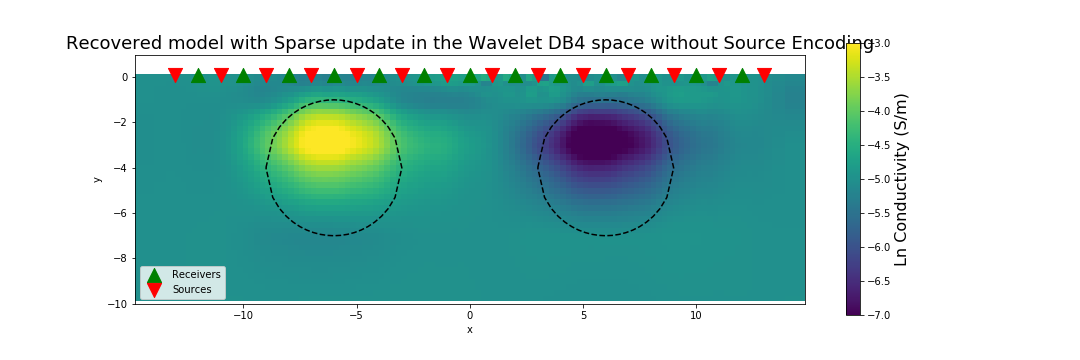
\includegraphics[width=59mm]{figures/recoveredModel_SparseWVT_DB4_withoutW.png}}
\end{figure}
\end{frame}

\begin{frame}{Coherency of J and Wavelet transform}
\begin{columns}
\begin{column}{0.6\textwidth}
\begin{figure}
  \subfigure{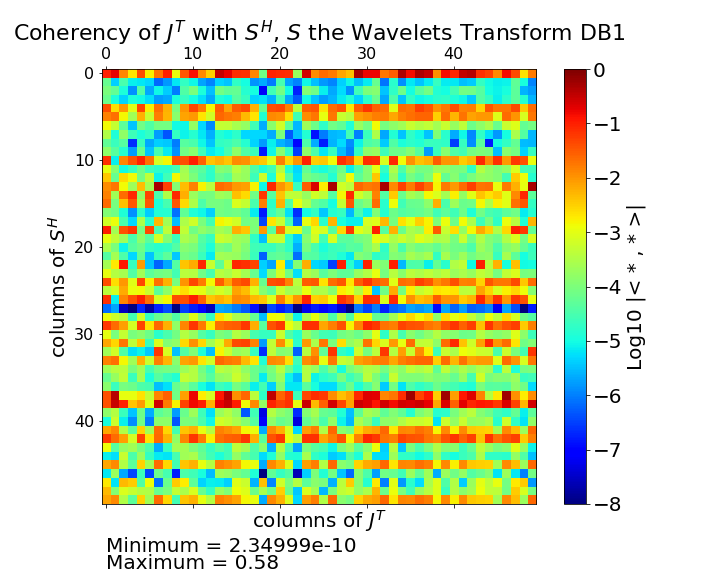
\includegraphics[width=30mm]{figures/Coherency_Wavelet.png}}
  \subfigure{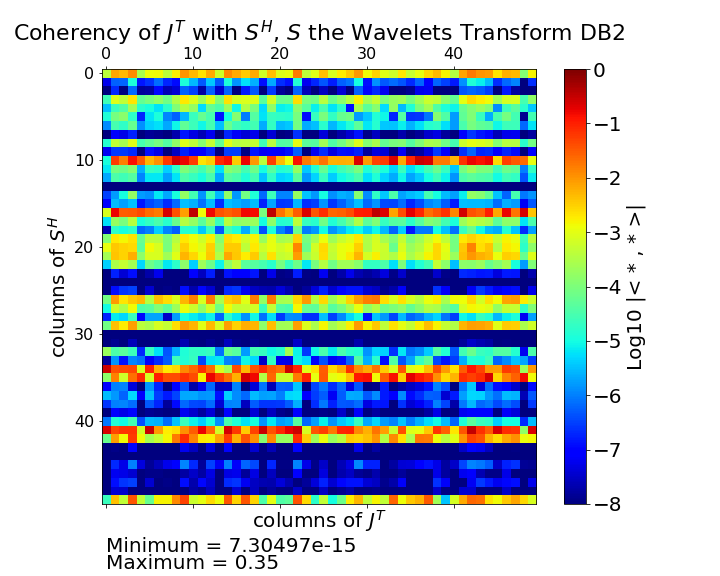
\includegraphics[width=30mm]{figures/Coherency_WaveletDB2.png}} \\
  \subfigure{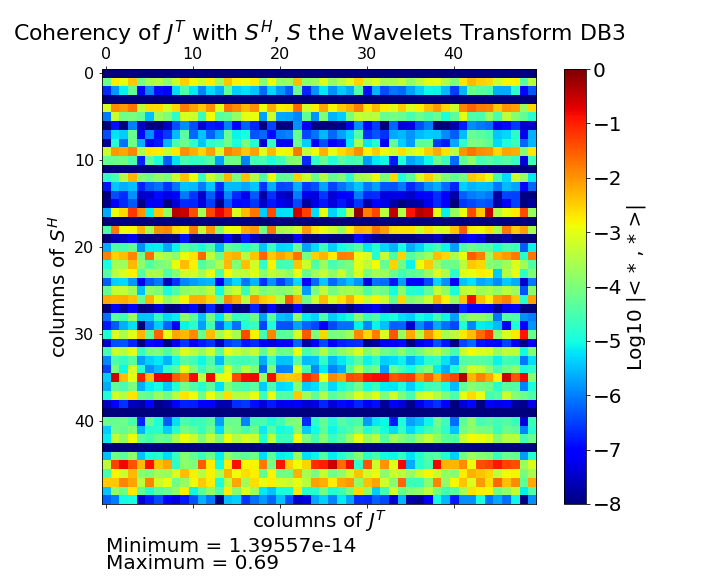
\includegraphics[width=30mm]{figures/Coherency_WaveletDB3.png}}
  \subfigure{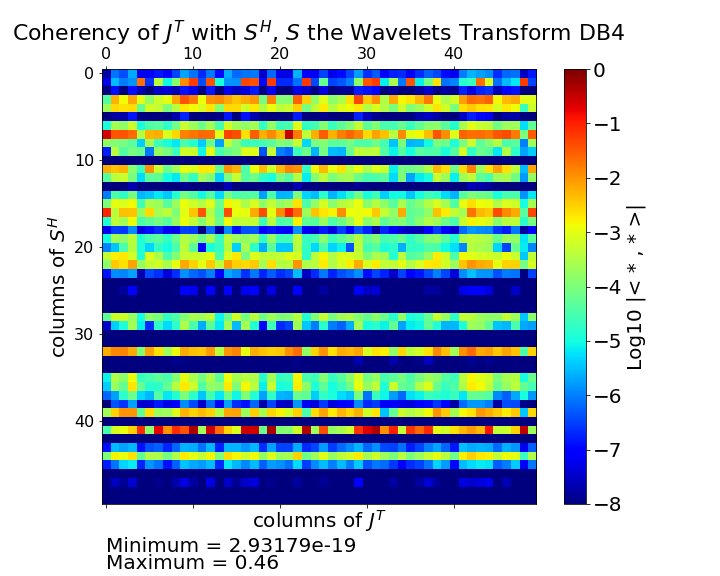
\includegraphics[width=30mm]{figures/Coherency_WaveletDB4.png}}
\end{figure}
\end{column}
\begin{column}{0.4\textwidth}
Possible explanation (hypothesis): asymptotic Incoherence \\
{\color{gray}Adcock, Ben, et al. "Breaking the coherence barrier: A new theory for compressed sensing." Forum of Mathematics, Sigma. Vol. 5. Cambridge University Press, 2017.}
\end{column}
\end{columns}
\end{frame}

\begin{frame}{Recovered Models using sparse GN update and Simultaneous Sources}
\begin{itemize}
  \item With Source Encoding
\end{itemize}
\begin{figure}
  \subfigure{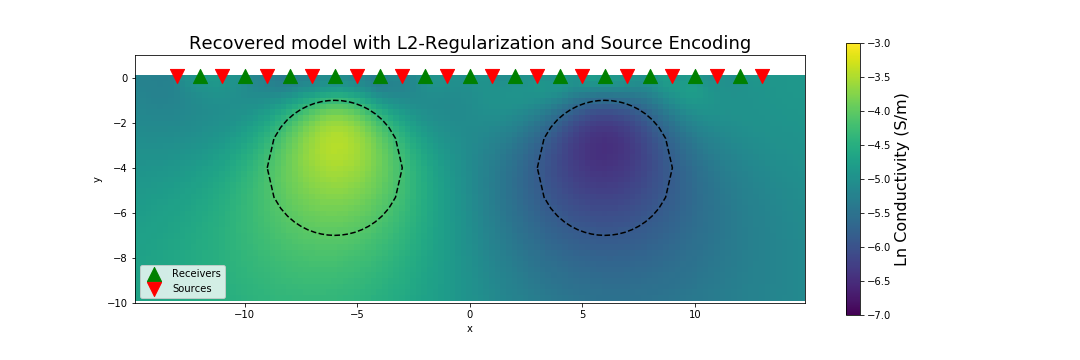
\includegraphics[width=59mm]{figures/recoveredModel_L2_withW.png}}
  \subfigure{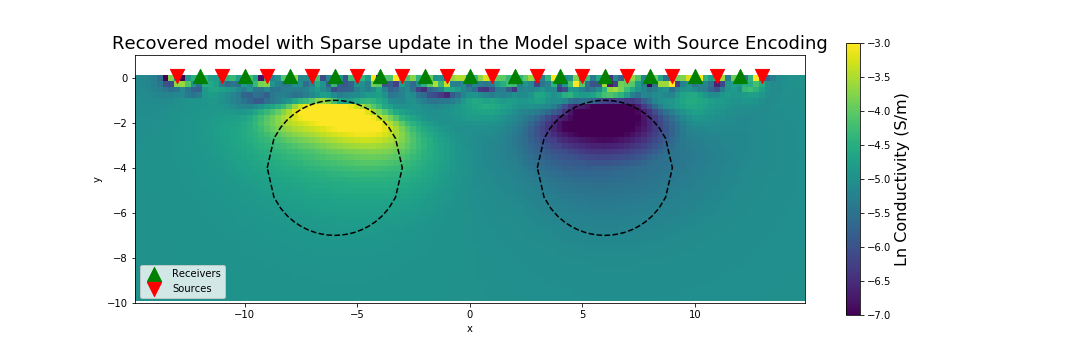
\includegraphics[width=59mm]{figures/recoveredModel_SparseId_withW.png}}
  \subfigure{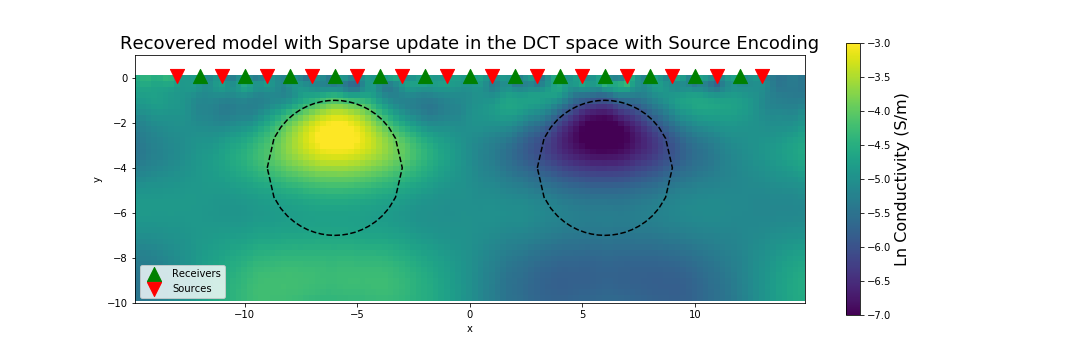
\includegraphics[width=59mm]{figures/recoveredModel_SparseDCT_withW.png}}
  \subfigure{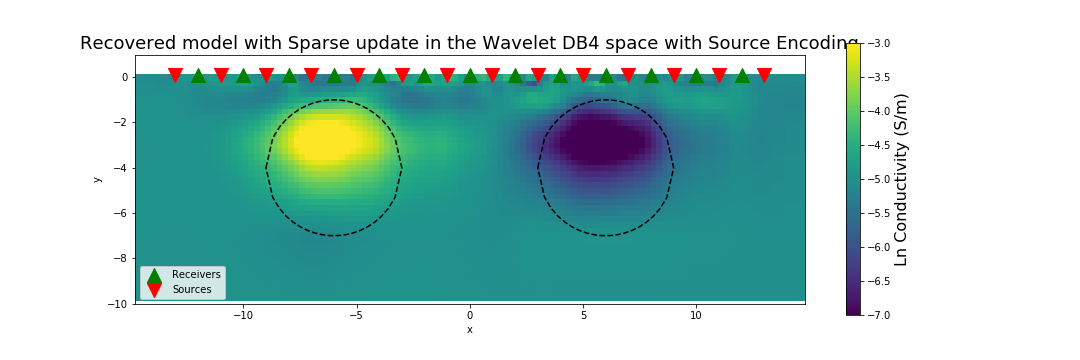
\includegraphics[width=59mm]{figures/recoveredModel_SparseWVT_DB4_withtW.png}}
\end{figure}
\end{frame}


\begin{frame}{Convergence Comparison}

\begin{figure}
  \subfigure{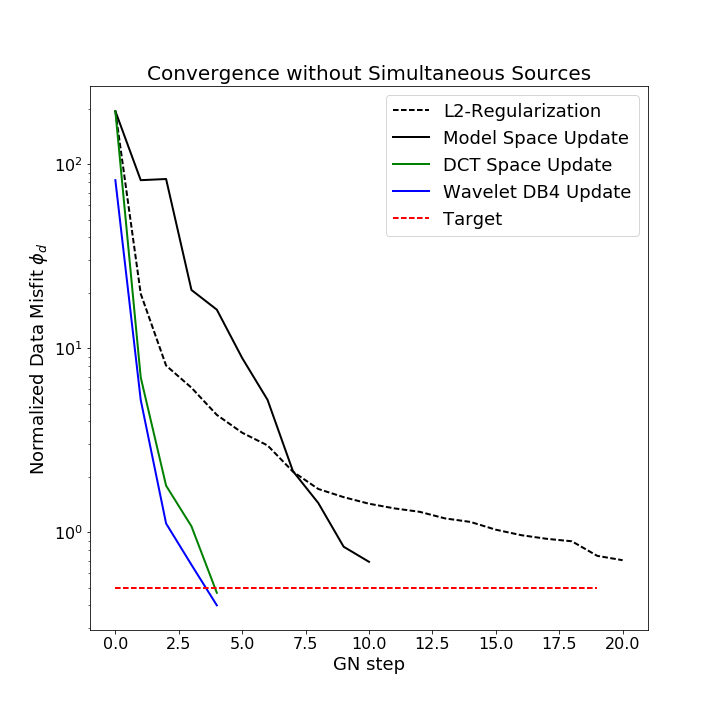
\includegraphics[width=49mm]{figures/Convergence_Sparse_withoutW.png}}
  \subfigure{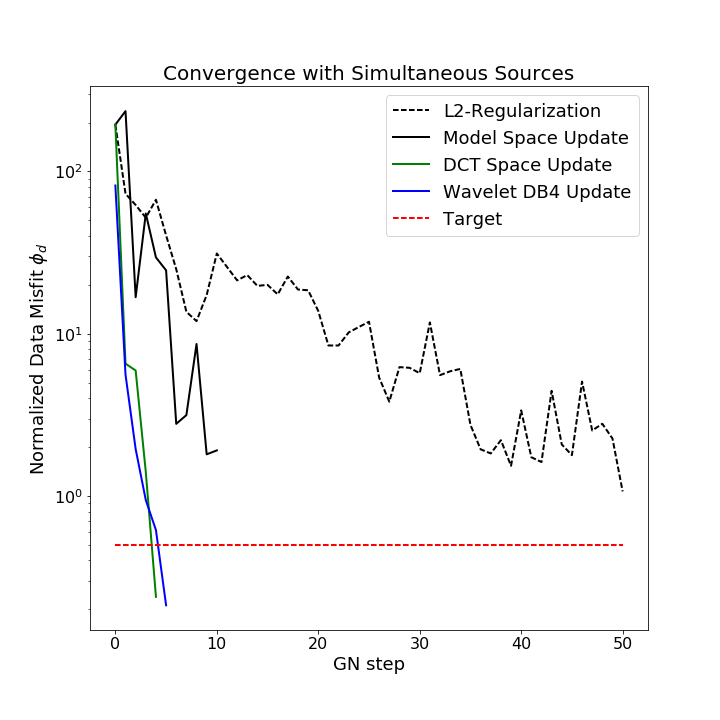
\includegraphics[width=49mm]{figures/Convergence_Sparse_withW.png}}
\end{figure}
\begin{itemize}
  \item L2 is still faster as each SPGL1 GN update is much more expansive to compute
  \item SPGL1 GN update seems even harder with Sim. Srcs!
\end{itemize}
\end{frame}



\begin{frame}{A curious behaviour}
\begin{itemize}
  \item Simulateneous Sources is killing the sparsity
\end{itemize}
\begin{figure}
  \subfigure{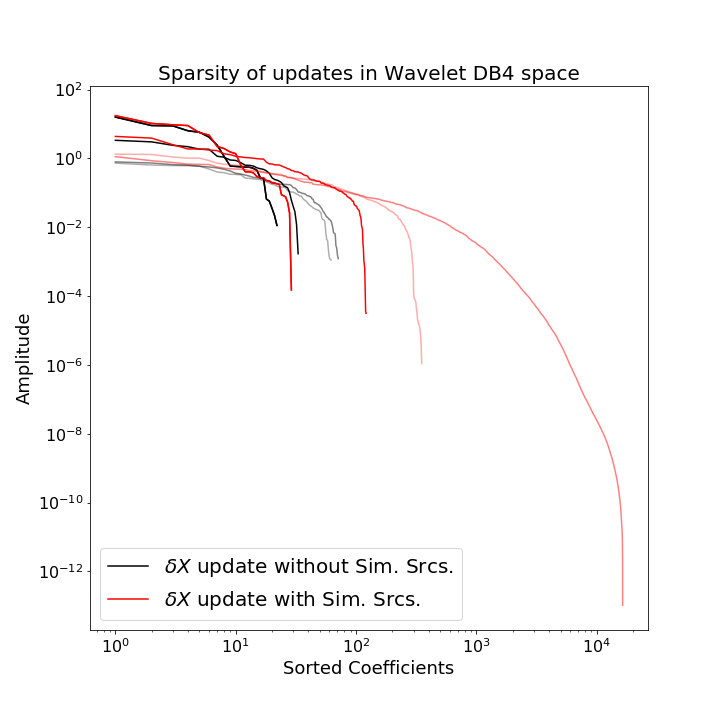
\includegraphics[width=39mm]{figures/SimSrc_kills_Sparsity_WVT_DB4.png}}
  \subfigure{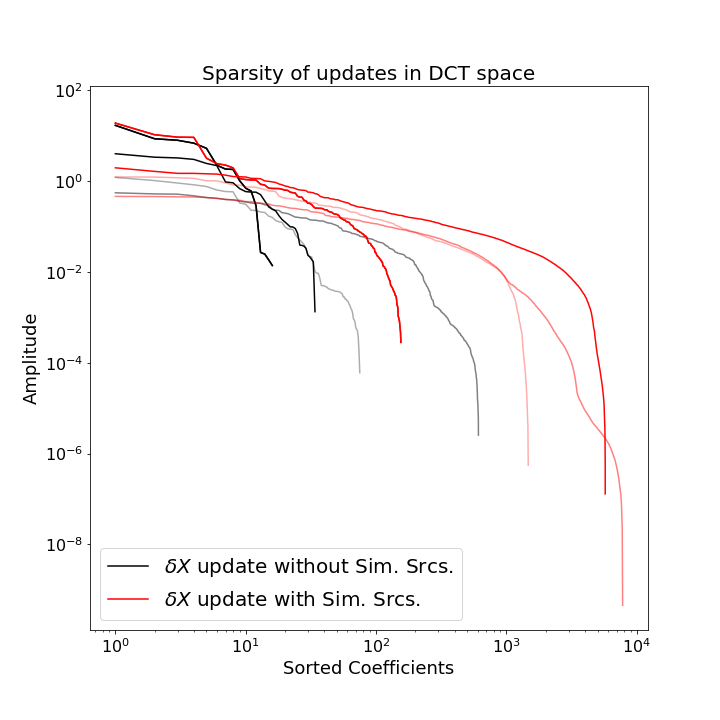
\includegraphics[width=39mm]{figures/SimSrc_kills_Sparsity_DCT.png}}
  \subfigure{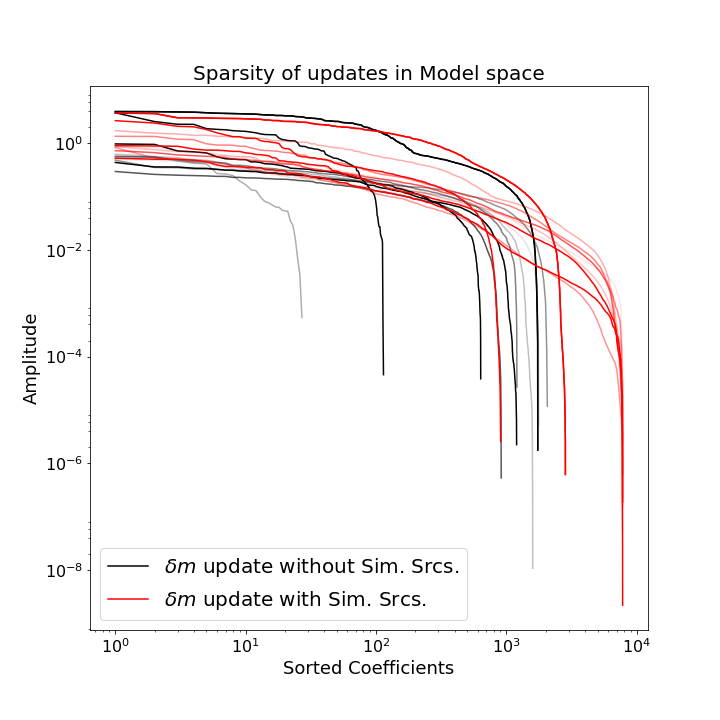
\includegraphics[width=39mm]{figures/SimSrc_kills_Sparsity_Id.png}}
\end{figure}

\end{frame}


\section{Discussion and Conclusion}

\begin{frame}{Discussion and Conclusion}
\begin{itemize}
  \item Simultaneous Sources
  \vspace{10pt}
  \begin{itemize}
    \item In terms of number of PDE solved for L2, the overall convergence rate is similar or worse
    \vspace{10pt}
    \item each step is a lot less memory-expansive, Useful if we have too many sources for our memory
    \vspace{10pt}
    \item for SPGL1, it has appeared to make things even worse, with longer time necessary to compute each GN update
  \end{itemize}
\end{itemize}
\end{frame}

\begin{frame}{Discussion and Conclusion}
\begin{itemize}
  \item Sparse GN Update
  \begin{itemize}
    \item At first, antagonization between sparsity in model space and the diffusive behavior of the Jacobian
    \vspace{3pt}
    \item Sparse update in model space are expansive to solve, sparse in DCT space is easier but recovered model is still smooth and display periodic patterns
    \vspace{3pt}
    \item Surprisingly, Wavelets have been an efficient transform despite a somehow high maximum for coherency
    \vspace{3pt}
    \item Simultaneous Sources has been a killer both for sparsity and computation times during our experiment
    \vspace{3pt}
    \item We did not study much the influence of the tolerance for the data fitting term in SPGL1 or the strategy to set it. Considering the time required for each iteration and the few iterations required to reach the target, we have probably been quite strict.
  \end{itemize}
\end{itemize}
\end{frame}


\begin{frame}

\begin{center}
{\Huge Thank you! \\}
\vspace{10pt}
All scripts and more are available on \href{https://github.com/thast/EOSC513}{\color{blue} Github/thast/} \\
\vspace{20pt}
Bonus: Another way to recover a compact model through prior information and vector quantization:
\end{center}

\begin{figure}
  \subfigure{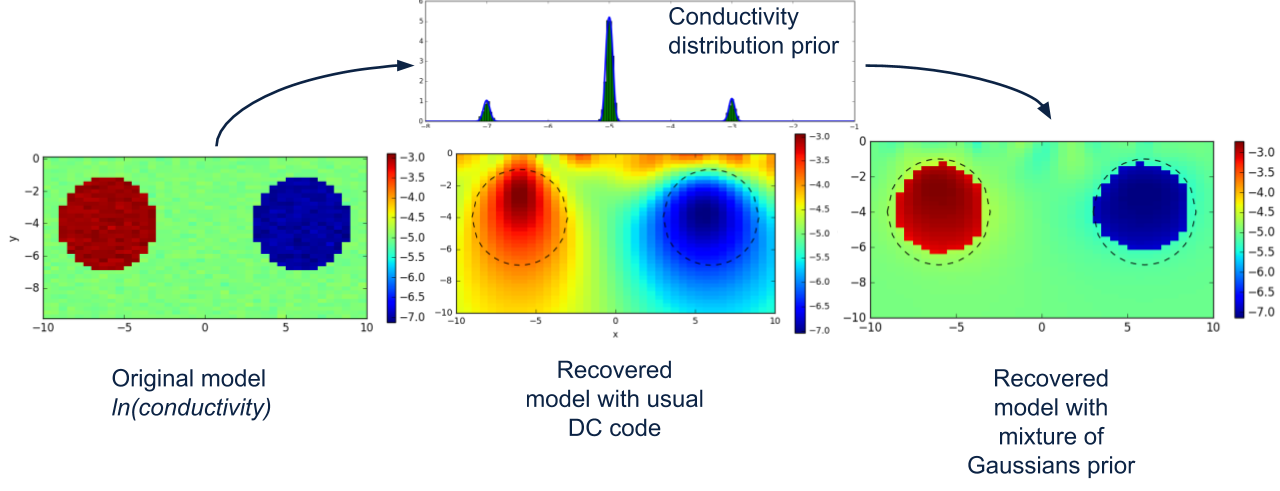
\includegraphics[width=80mm]{figures/ThibautAsticClusterAlgorithm_crop.png}}
\end{figure}

\end{frame}

\end{document}